\chapter{Implementation}
\section*{Introduction}
In this chapter, we describe the working environment used during
the implementation of our application. We will also describe its physical layout using a deployment diagram. Then, we
detail the work carried out and the results obtained using a set
of screenshots representing the interfaces of the different features of
our app.
\section{Technical specification}
In this section, we will present the technical choices relating to
the hardware and software environment that contributed to the realization of our
application.
\subsection{Hardware environment}
During the different stages of our project, i.e. documentation,
code implementation and testing, we had:
\begin{itemize}
\item A laptop computer with the following configuration:
\begin{itemize}
\item Brand: Lenovo;
\item Processor: AMD Ryzen 3 3200U @ 2.60 GHz ;
\item Graphical processor:  Radeon Vega Mobile Gfx;
\item RAM: 12 GB;
\item Hard disk: 1TB;
\item System type: Windows 64-bit operating system.
\end{itemize} 
\item A desktop computer with the following characteristics:
\begin{itemize}
\item Brand: Lenovo;
\item Processor: Intel(R) Core(TM) i3-7100 CPU @ 3.90GHz 3.91GHz ;
\item Graphical processor: NVIDIA GeForce GT 1030
\item RAM: 8 GB;
\item Hard disk: 500 GB + 300 GB;
\item System type: Windows 64-bit operating system.
\end{itemize}
\end{itemize}
\subsection{Software environment}
Throughout the development phase, we used these software tools
and the following programming languages and frameworks:
\subsubsection{Software tools}
During the implementation of our project, we used the following software :
\paragraph*{Visual Studio Code}
Visual Studio Code is a popular source code editor developed by Microsoft. It provides a powerful and customizable environment for software development across various programming languages. Known for its lightweight design and extensive plugin ecosystem, Visual Studio Code offers features such as syntax highlighting, code completion, debugging capabilities, and version control integration. It supports multiple operating systems and offers a user-friendly interface.\\
Visual Studio Code allows mainly the JS/HTML/CSS files in our application as well as the XML configuration files for each LWC component, in addition to Cls files that represent the Apex Controllers and the files representing the Aura applications.
\begin{figure}[H]%
    \center   
    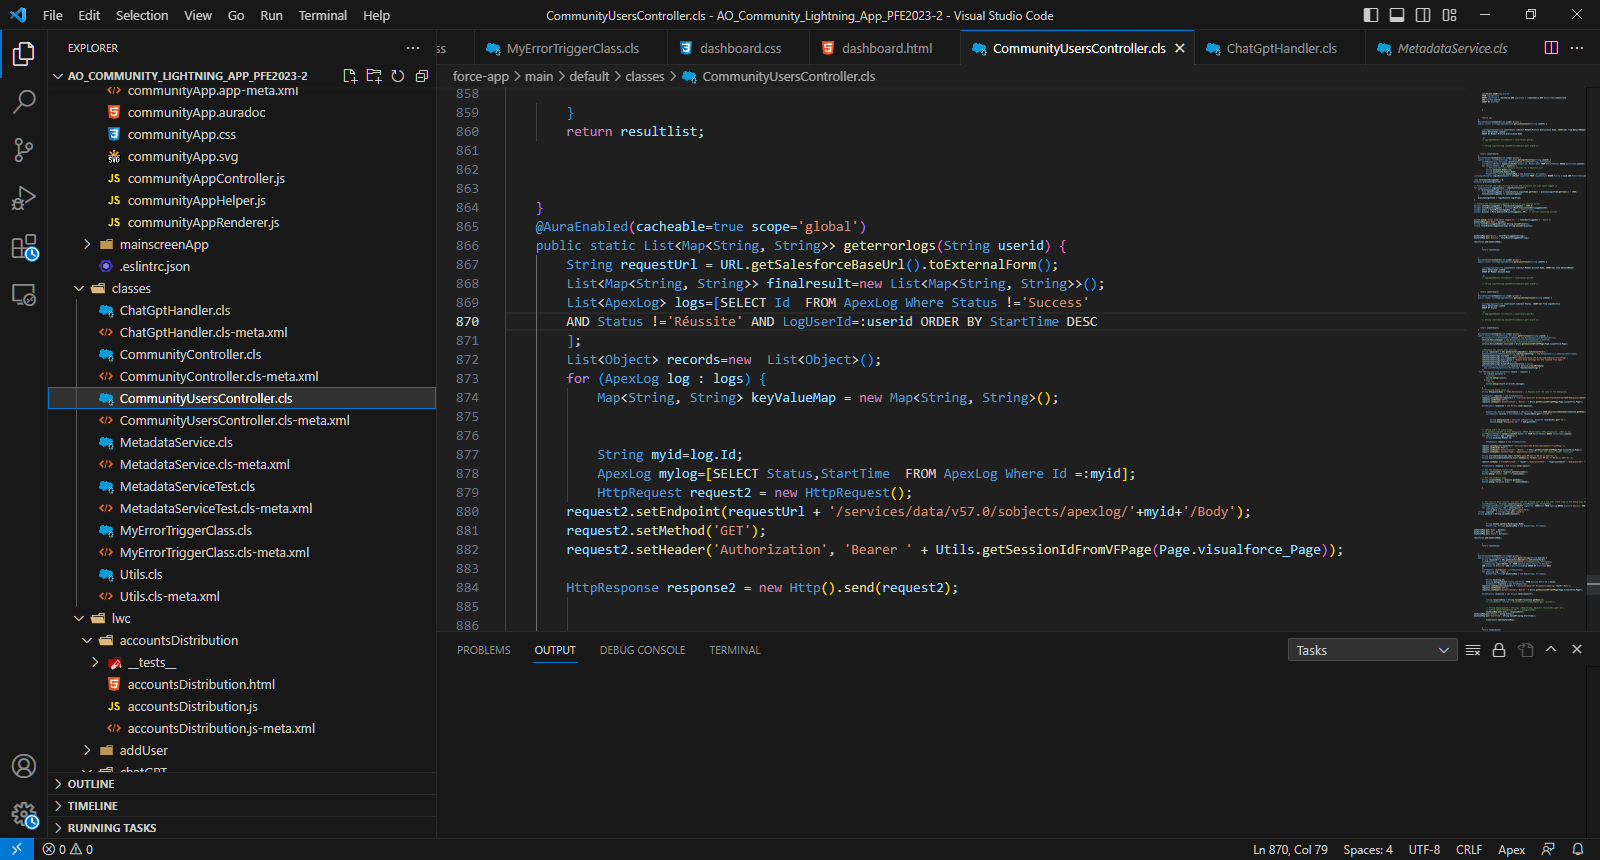
\includegraphics[scale=0.4]{vs.png}
    \caption{Visual Studio Code}
\end{figure}
\paragraph*{Salesforce Extension Pack for Visual Studio Code}
The Salesforce Development Extension Pack offers a collection of powerful tools specifically designed for developers working on the Salesforce platform. Integrated seamlessly with the lightweight and highly extensible VS Code editor, these tools empower developers with a comprehensive set of features tailored for various aspects of Salesforce development. With specialized functionalities for managing development orgs, including scratch orgs, sandboxes, and DE orgs, as well as robust support for Apex, Aura components, and Visualforce, the extension pack significantly enhances the development experience and productivity for Salesforce developers.
\begin{figure}[H]%
    \center   
    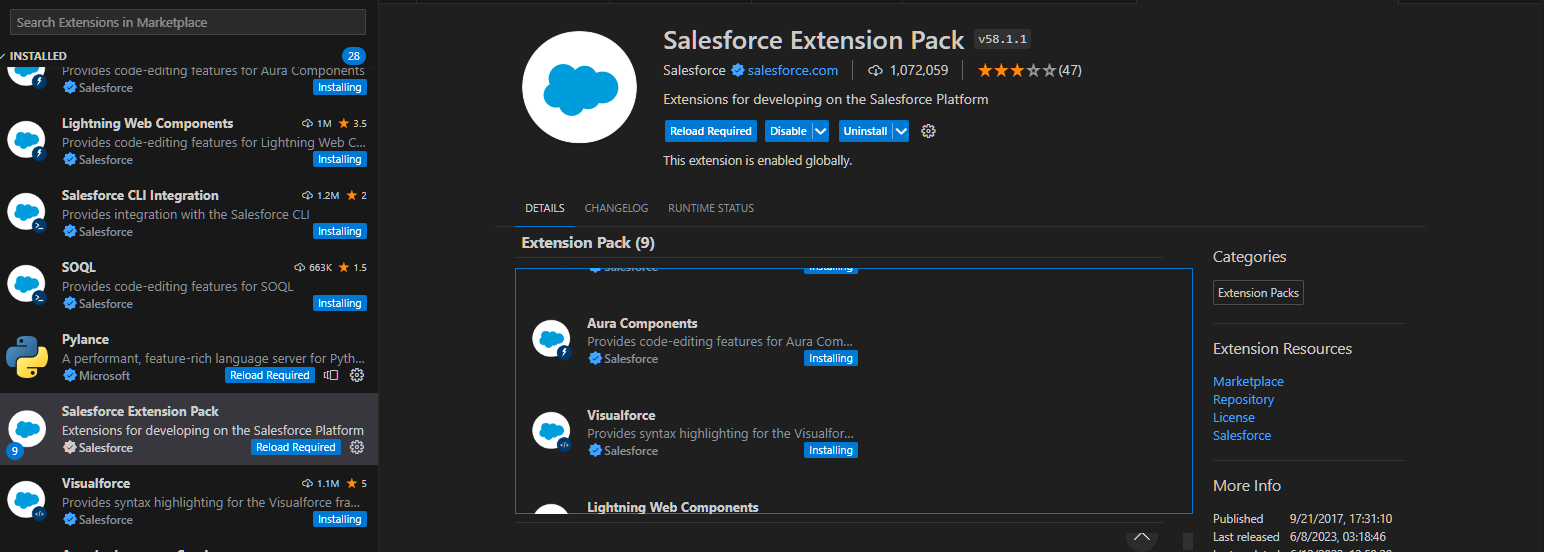
\includegraphics[scale=0.4]{extensions.png}
    \caption{Salesforce Extension Pack }
\end{figure}
\paragraph*{Salesforce CLI (sfdx)}
The Salesforce CLI is an essential command line interface that streamlines the development and automation processes for Salesforce orgs. It offers a wide range of capabilities, allowing developers to:
\begin{itemize}

\item[•] Consolidate Development Tools: By utilizing the Salesforce CLI, developers can bring together all the necessary tools required for efficient development and execute commands seamlessly within their Salesforce org.

\item[•] Source Synchronization: The CLI enables developers to synchronize source code between local environments and scratch orgs, ensuring that changes made in the development environment are accurately reflected in the org.

\item[•] Org Management: Developers can create and manage orgs effortlessly using the CLI. This includes provisioning new orgs, configuring various settings, and handling administrative tasks.

\item[•] Data Import and Export: With the CLI, developers can easily import and export data to and from their Salesforce orgs, facilitating data migration, data backup, and data integration processes.

\item[•] Test Creation and Execution: The CLI provides functionalities for creating and executing tests, allowing developers to ensure the quality and reliability of their code through automated testing procedures.

\item[•] Package Creation and Installation: Developers can utilize the CLI to create packages that encapsulate specific components or functionalities within their Salesforce orgs. These packages can be easily installed in other orgs, simplifying the deployment and distribution of applications.
\end{itemize}

\begin{figure}[H]%
    \center   
    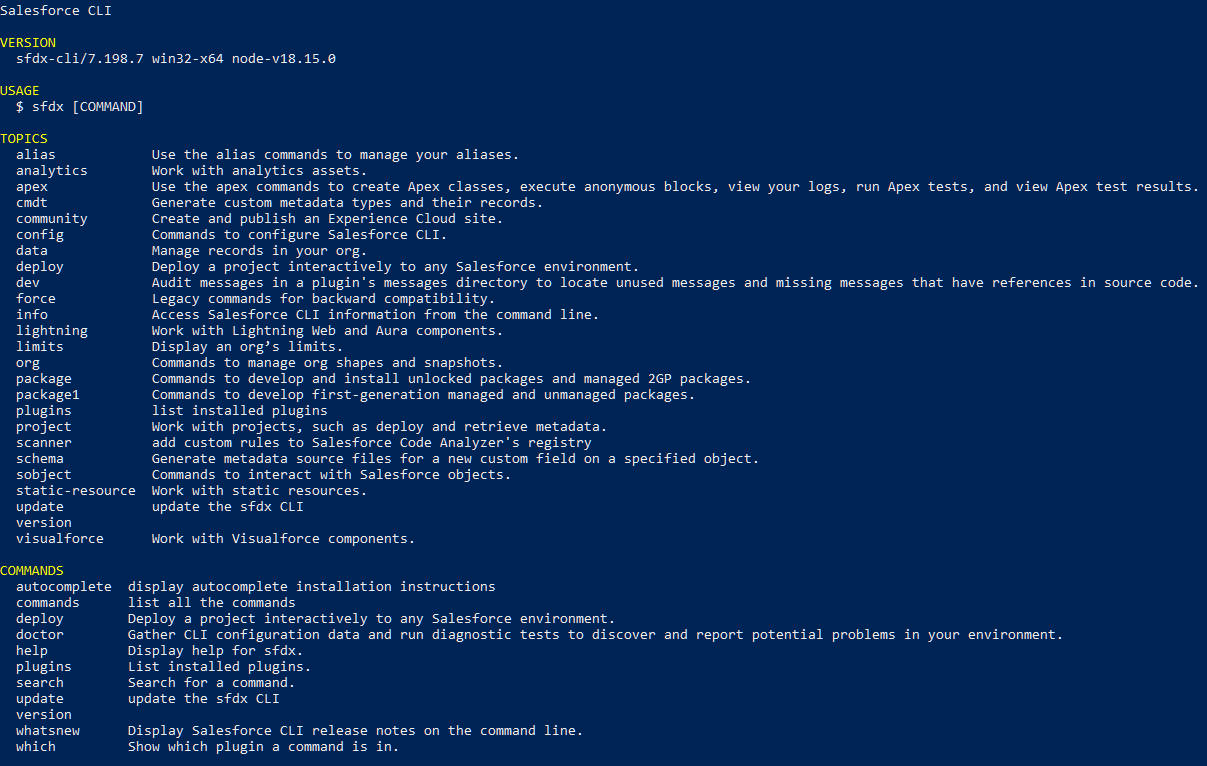
\includegraphics[scale=0.4]{cli.png}
    \caption{Salesforce CLI}
\end{figure}

\paragraph*{Salesforce Inspector}
Salesforce Inspector is a highly useful productivity tool designed specifically for Salesforce administrators and developers. It offers the capability to inspect data and metadata directly within the Salesforce user interface (UI), enhancing the efficiency and convenience of working with Salesforce.
With the added metadata layout, we were able to gain enhanced visibility and control over our Salesforce environment, making it easier to navigate, manipulate, and analyze data and metadata that is hidden by usual means.

\begin{figure}[H]%
    \center   
    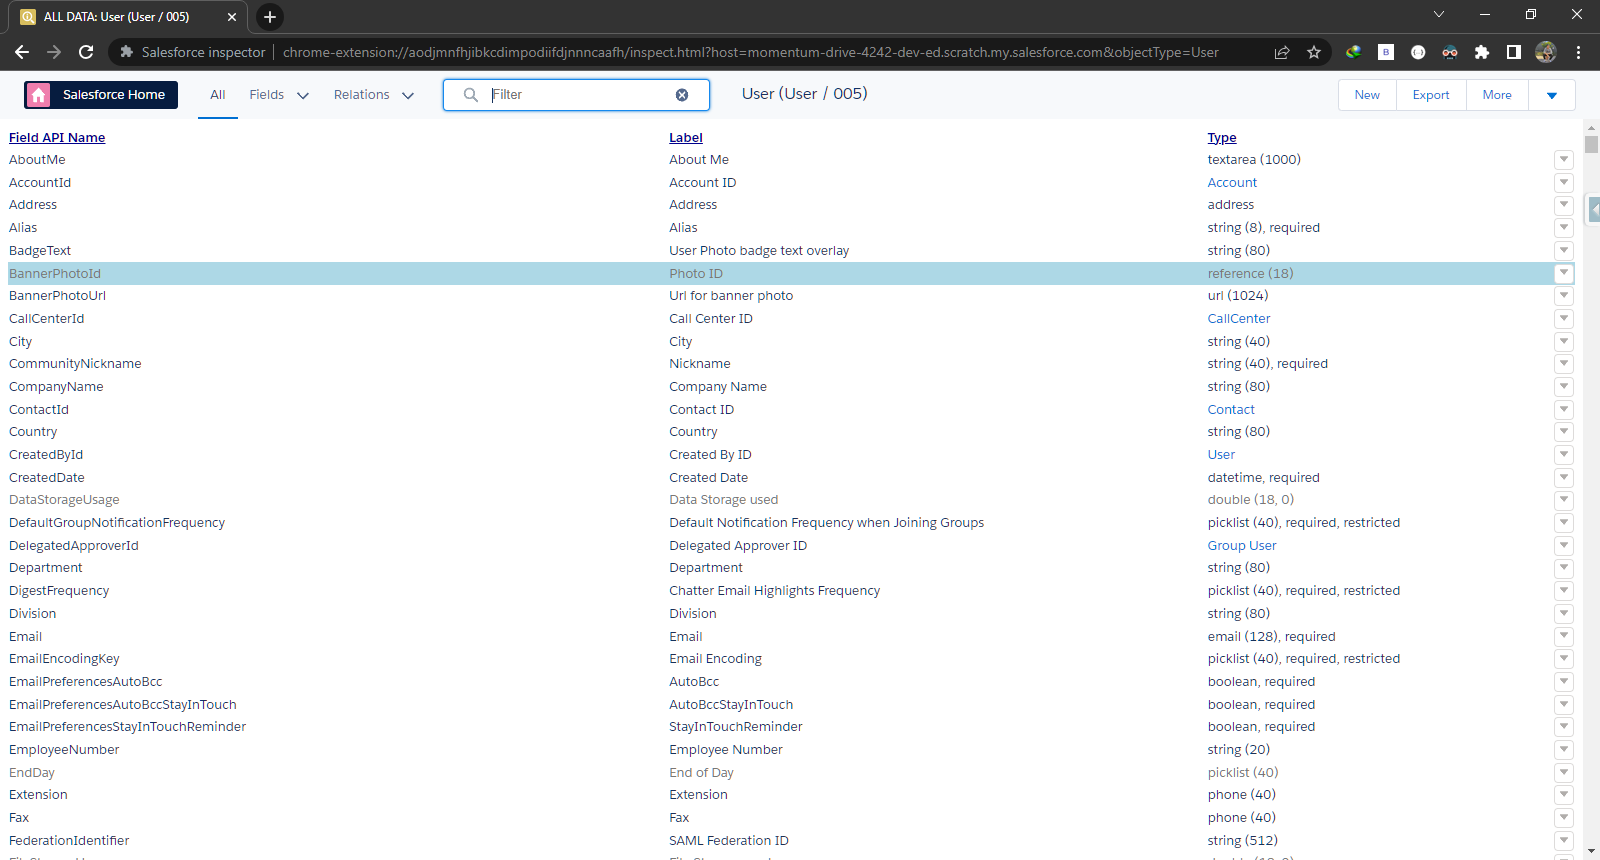
\includegraphics[scale=0.4]{inspector.png}
    \caption{Salesforce Inspector}
\end{figure}

\paragraph*{Maven Tools for Salesforce}
Maven Tools is an all-encompassing collection of Salesforce developer tools, purposefully designed to cater to the needs of Salesforce technical consultants. With its unique architecture, Maven Tools revolutionizes the delivery process of Salesforce implementations. This comprehensive toolkit offers a wide range of features, including an intelligent query editor, REST console, event hub, and much more, empowering developers to execute changes with increased speed and effectiveness.\\
In our application, we used Maven Tools for accessing the Salesforce tooling API.

\begin{figure}[H]%
    \center   
    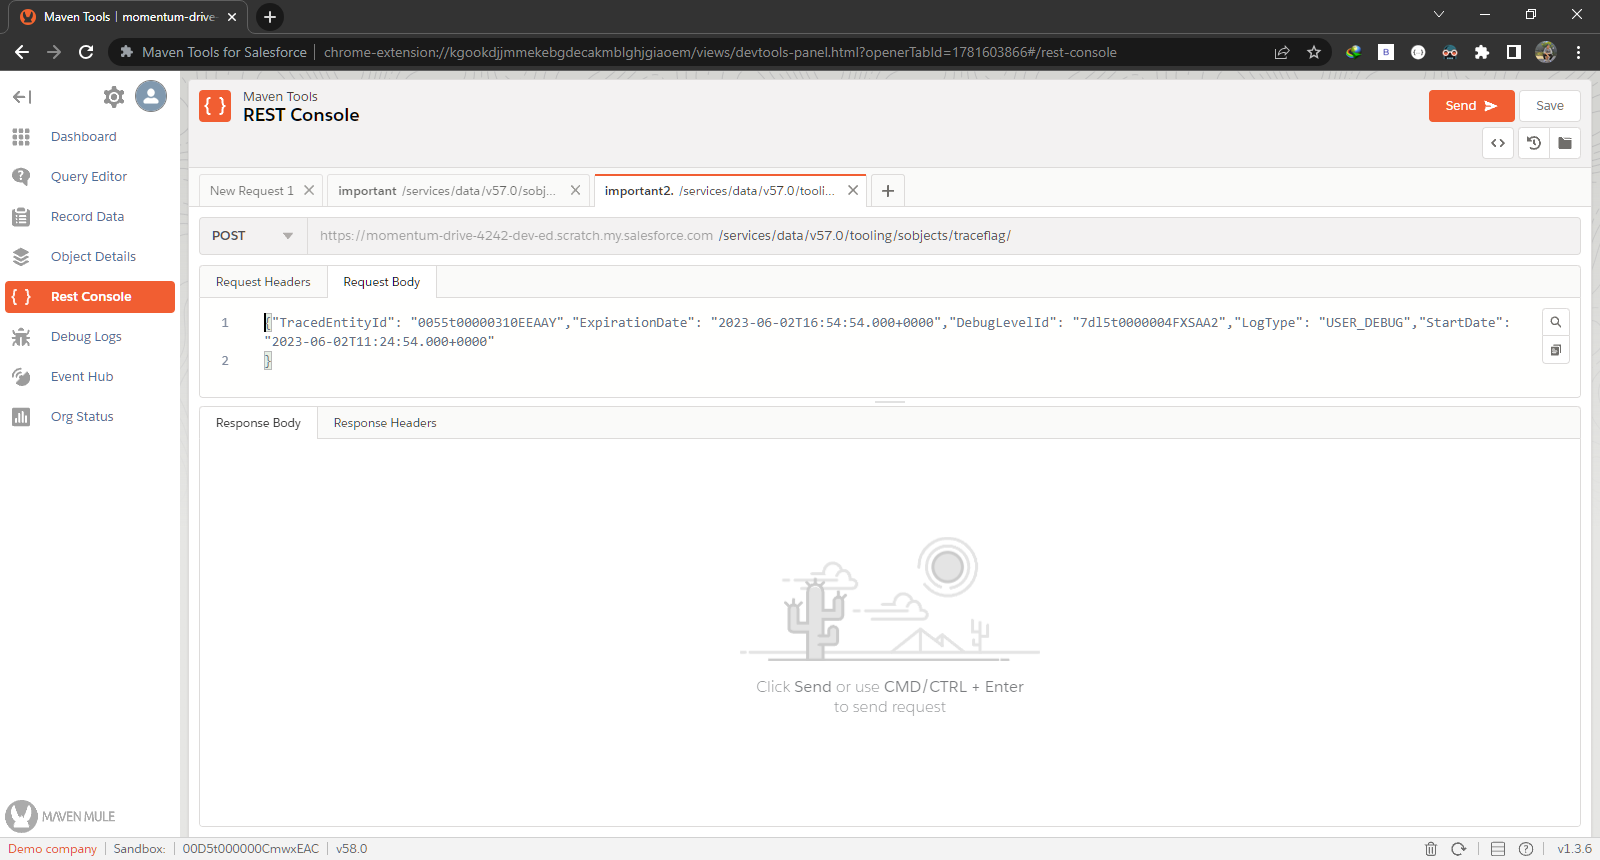
\includegraphics[scale=0.4]{maven.png}
    \caption{Maven Tools}
\end{figure}

\paragraph*{StarUML}
StarUML is a versatile software engineering tool designed for system modeling, employing various modeling notations including the Unified Modeling Language (UML), Systems Modeling Language (SysML), and classical modeling notations. Developed and published by MKLabs, StarUML offers comprehensive modeling capabilities and is compatible with Windows, Linux, and macOS operating systems.\\
In our application, we used StarUML to establish UML diagrams for this report.
\begin{figure}[H]%
    \center   
    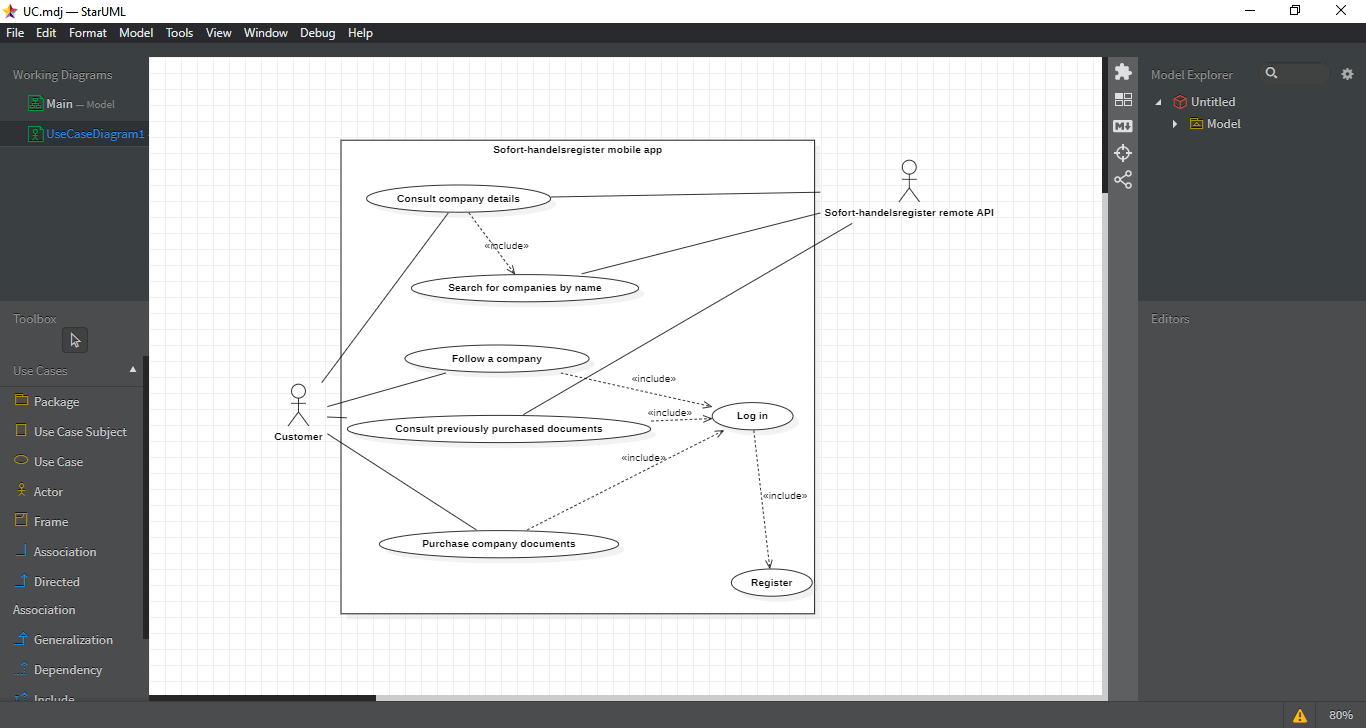
\includegraphics[scale=0.4]{star.png}
    \caption{StarUML}
\end{figure}
%current progress
\subsubsection{APIs and libraries}
\paragraph*{Salesforce Tooling API}
The Tooling API is a valuable resource for developers looking to create custom development tools or applications for Lightning Platform applications. It offers a range of capabilities that facilitate efficient and interactive development experiences.
One of the advantages of the Tooling API is its ability to retrieve smaller pieces of metadata using SOQL (Salesforce Object Query Language). This enables developers to fetch specific metadata components, resulting in improved performance compared to retrieving larger sets of metadata. \\
In our application, Salesforce tooling API was used to enable our application to interact with private Salesforce objects like Traceflag and DebugLevel.

\paragraph*{OpenAI API}
The OpenAI API is a versatile tool that can be utilized for a wide range of tasks involving natural language understanding and generation, as well as code-related operations. With its capabilities, the OpenAI API enables users to perform tasks such as language translation, text summarization, sentiment analysis, ChatBot development, and more.\\
In our application, OpenAI API was used to power up our Salesforce digital assistant and enable it to understand natural language.

\paragraph*{Libraries}
\begin{table}[H]
\begin{tabular}{|l|l|}
\hline
\textbf{Library}                                                       & \textbf{Usage}                                                                                                                                                                     \\ \hline
\begin{tabular}[c]{@{}l@{}}Salesforce \\ Metadata Service\end{tabular} & \begin{tabular}[c]{@{}l@{}}- Automate remote site settings configuration.\\ - Automate custom Salesforce object for chatbot feedback.\end{tabular}                                 \\ \hline
LWC's wire                                                             & \begin{tabular}[c]{@{}l@{}}- Establish a connection between the lightning web component \\ and an Apex method, a function in a JavaScript module, or a wire adapter.\end{tabular} \\ \hline
LWC's API & - Create a public property or method that can be accessed by parent components.                                                                                                    \\ \hline
Chart Js                                                               & - Build responsive and interactive charts from given Salesforce data.                                                                                                              \\ \hline
\end{tabular}
\caption{Libraries}
\end{table}
\subsubsection{Programming languages and frameworks}
\paragraph*{Apex}
Apex is a strongly typed, object-oriented programming language that allows developers to execute flow and transaction control statements on Salesforce servers in conjunction with calls to the API. Using syntax that looks like Java and acts like database stored procedures, Apex enables developers to add business logic to most system events, including button clicks, related record updates, and Visualforce pages. Apex code can be initiated by Web service requests and from triggers on objects.\cite{8}
\paragraph*{LWC(Lightning Web Components)}
Lightning Web Components is a framework that leverages core Web Components standards and focuses on delivering optimal performance within Salesforce-supported browsers. By utilizing the native capabilities of modern browsers, Lightning Web Components achieves a lightweight structure that excels in performance. It primarily utilizes standard JavaScript, HTML, and CSS, making it accessible and familiar to those already experienced in web development.
\paragraph*{Aura}
Aura components are the self-contained and reusable units of an app. They represent a reusable section of the UI and can range in granularity from a single line of text to an entire app.
The framework includes a set of prebuilt components. For example, components that come with the Lightning Design System styling are available in the lightning namespace.\cite{9}
\paragraph*{SOQL}
SOQL (Salesforce Object Query Language) serves as a powerful query language dedicated to retrieving data from Salesforce databases. While sharing similarities with SQL (Structured Query Language), SOQL is specifically designed for querying Salesforce data.
Using SOQL, developers can efficiently query and retrieve data from both standard and custom objects within the Salesforce platform. This includes accessing records, and fields, and establishing relationships between different objects. 
\paragraph*{SLDS}
The Salesforce Lightning Design System (SLDS) represents a comprehensive set of guidelines and resources offered by Salesforce to easily create visually consistent and user-friendly interfaces within Salesforce applications.
It also provides developers with a rich assortment of CSS styles, design patterns, and components. These resources can be utilized to construct custom Salesforce applications, including Lightning Web Components (LWC) and Aura components.
\paragraph*{XML}
The XML (Extensible Markup Language) allows the developer to create and share information formats via networks. This standard is used to describe data in our application as well as configure component visibility in Salesforce.
\paragraph*{JSON}
JSON(JavaScript Object Notation) is a lightweight data-interchange format that is easy to read and write and
frequently used by developers. Within our application, it was mainly used for communicating with external APIs. 
\subsection{Deployment diagram of the application}
The deployment diagram models the physical architecture of a system.
This diagram shows the topology of the software elements that are deployed over the material elements.
The following figure represents the deployment diagram of our application.
\begin{figure}[H]%
    \center   
    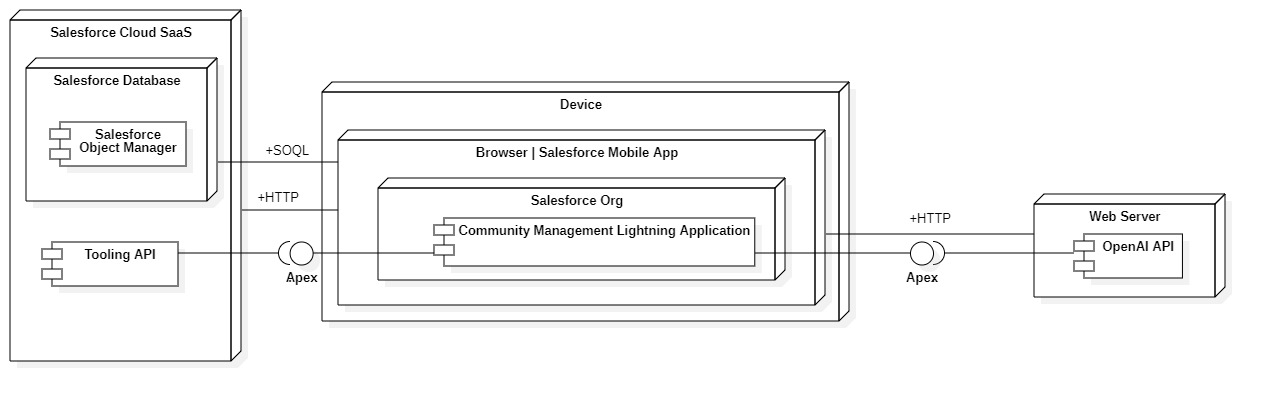
\includegraphics[scale=0.4]{DeploymentDiagram.jpg}
    \caption{Deployment diagram of the application}
\end{figure}
Our application's deployment diagram is composed of 3 Nodes:
\begin{itemize}
\item Device: the physical device that is used to access the user's Salesforce org containing our lightning application
\item Web Server: the web server embedding the OpenAI API responsible for powering up our ChatBot 
\item Salesforce cloud SAAS(software as a service): the provider of the Salesforce database that enables our application to create, read, update, or delete Salesforce records' data and the provider of the tooling API that enables our application to automate org configuration and similar operation.  
\end{itemize}
The interactions between software components are:
\begin{itemize}
\item[•] between our application and OpenAI API via HTTP requests. The exchange of data is in JSON format through the
REST(representational state transfer) APIs, the resulting data is exploited through Apex.
\item[•] between our application and Salesforce Database via SOQL queries. The exchange of data is in sObjects (Salesforce objects) format.
\item[•] between our application and Tooling API via HTTP requests. The exchange of data is in JSON format through the
REST(representational state transfer) APIs, the resulting data is exploited through Apex.

\end{itemize}

\section{Application interfaces}
In this part, we present the different features of our
application by presenting the graphical interfaces produced:
\subsection{Launching the application}
The following figure represents the landing page of the application where the user can choose to access one of his owned communities or search for a specific one by its name using the provided search bar.
\begin{figure}[H]%
    \center   
    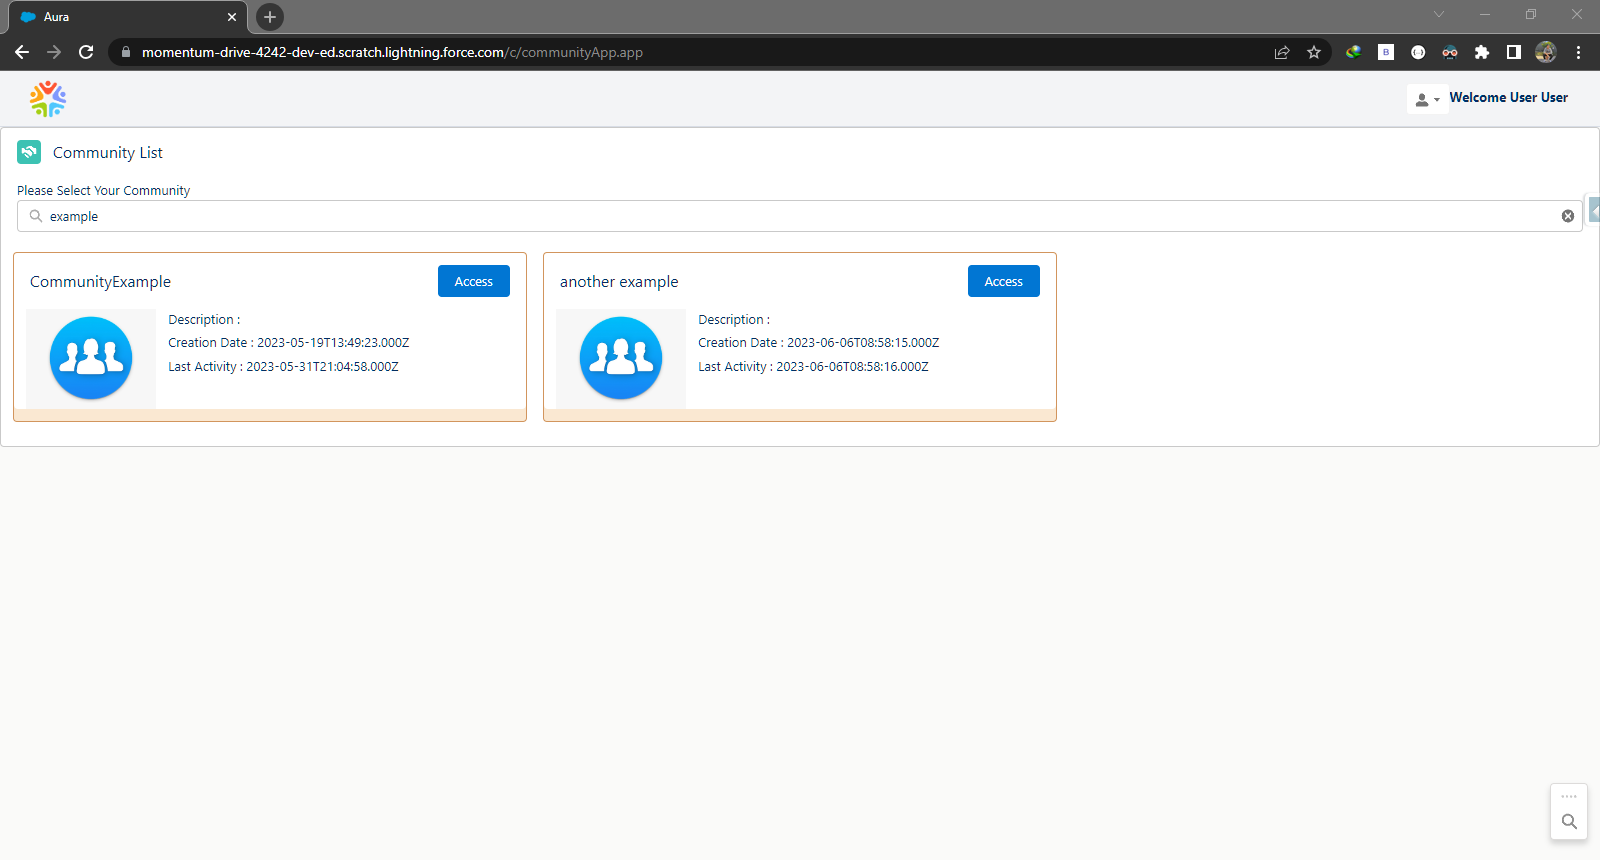
\includegraphics[scale=0.4]{home.png}
    \caption{Community selection interface (landing page of the application)}
\end{figure}
\subsection{Community Dashboard}
The following figure represents the community dashboard, that shows up upon accessing the selected community bu the user, containing KPIs charts that help the user monitor his community.\\
The following figure represents respectively the accounts distribution chart, Salesforce user licenses distribution chart, and login attempts status distribution chart for the current community.
\begin{figure}[H]%
    \center   
    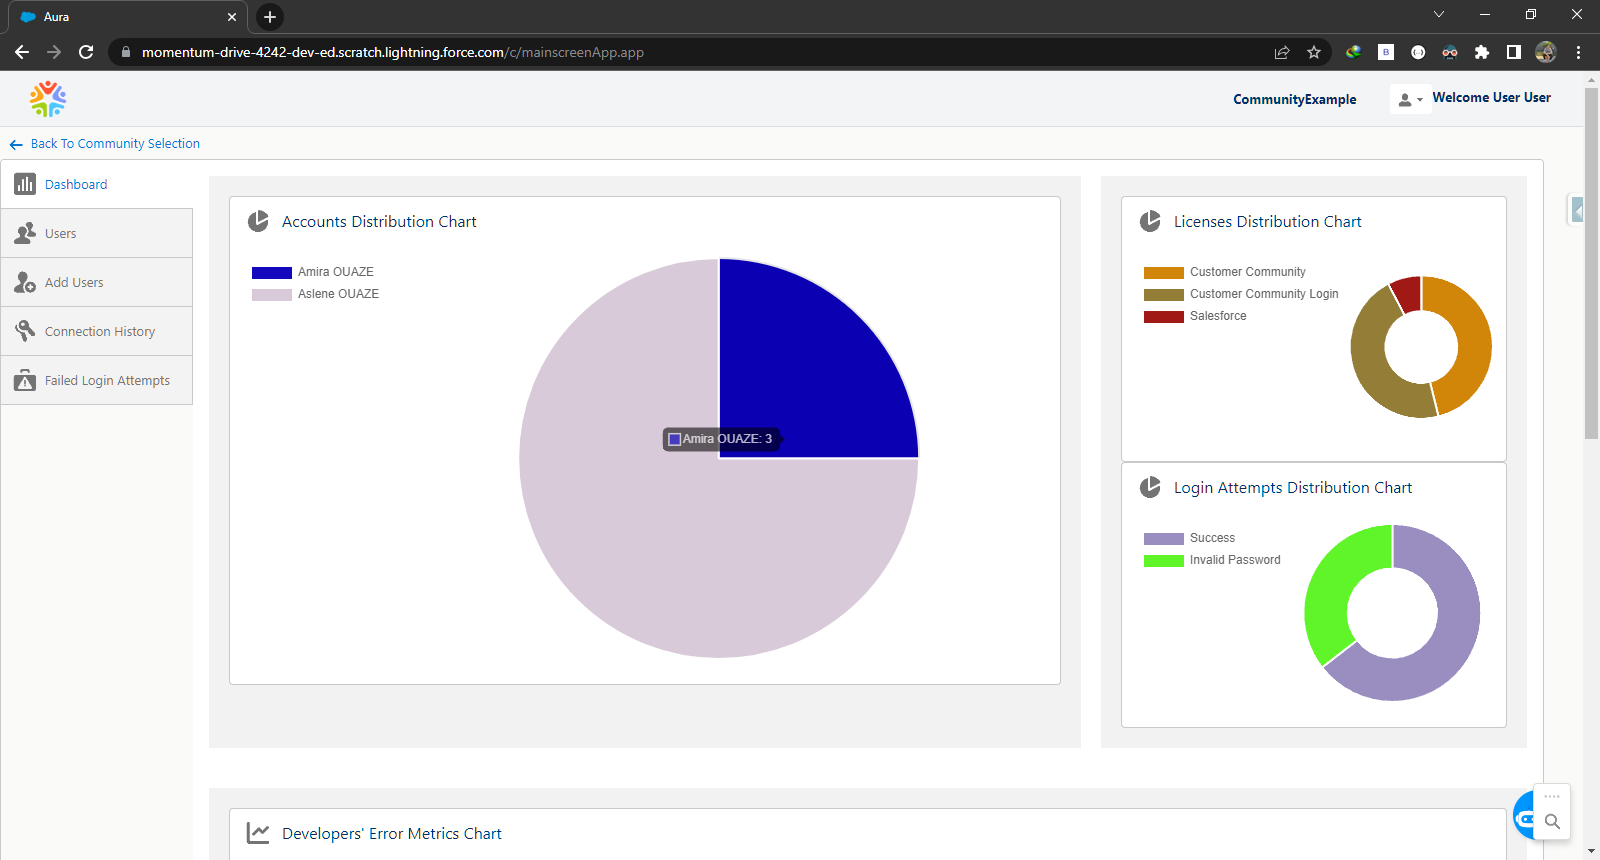
\includegraphics[scale=0.4]{dashboard1.png}
    \caption{Community dashboard interface (distribution charts)}
\end{figure}
The following figure represents the time spent in the community chart that shows the number of hours and minutes spent by each member when surfing the current community.
\begin{figure}[H]%
    \center   
    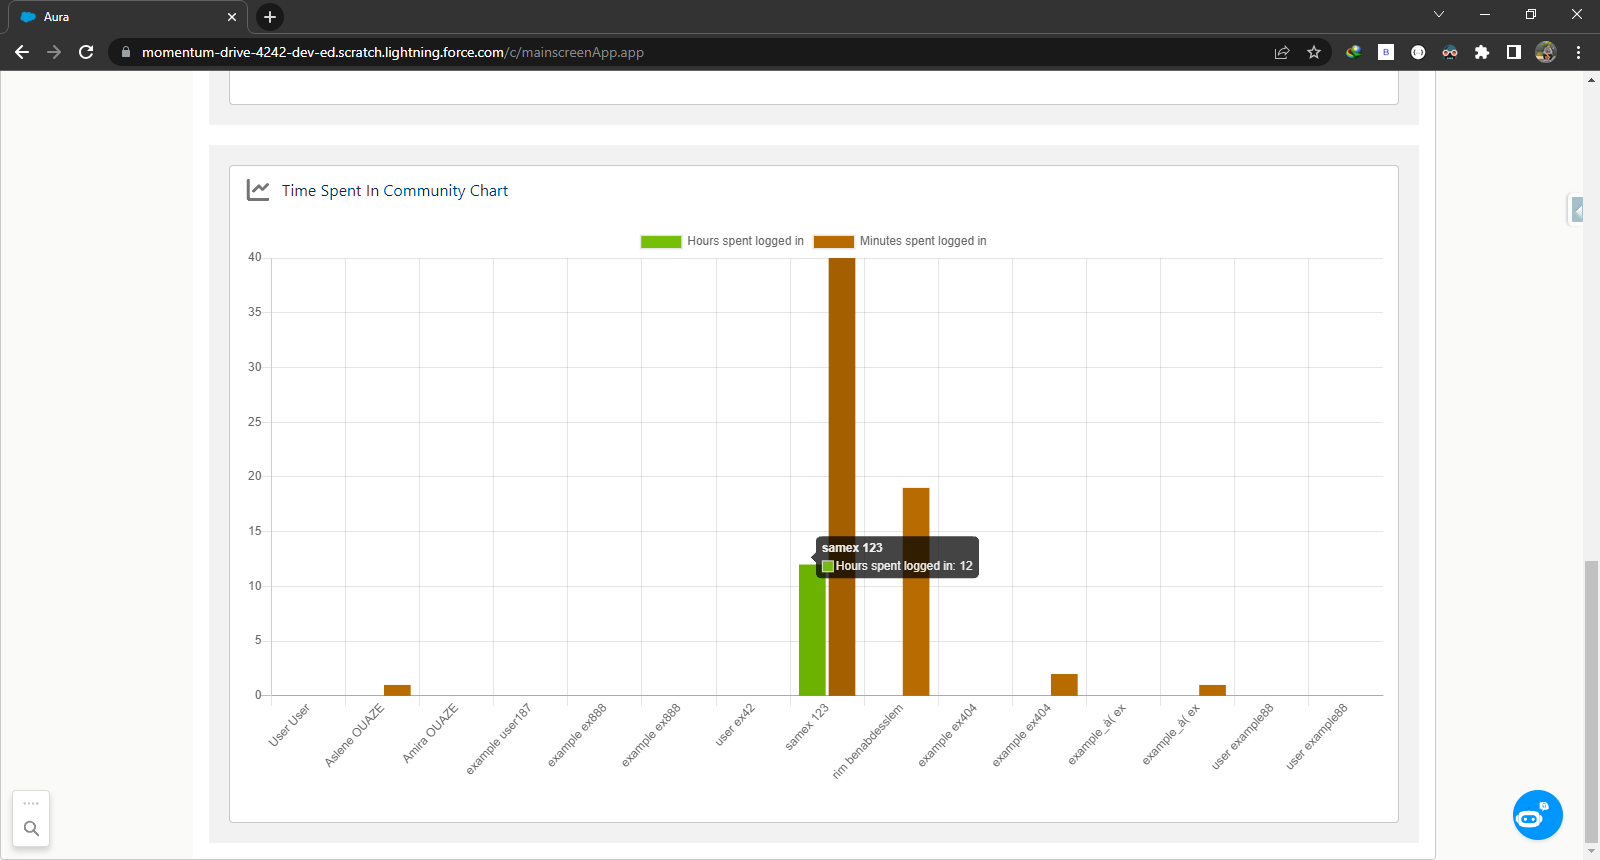
\includegraphics[scale=0.4]{dashboard2.png}
    \caption{Community dashboard interface (time spent in the community chart)}
\end{figure}
The following figure represents the community developers' error metrics chart that shows the number of programming errors faced by each developer working in the current community.
\begin{figure}[H]%
    \center   
    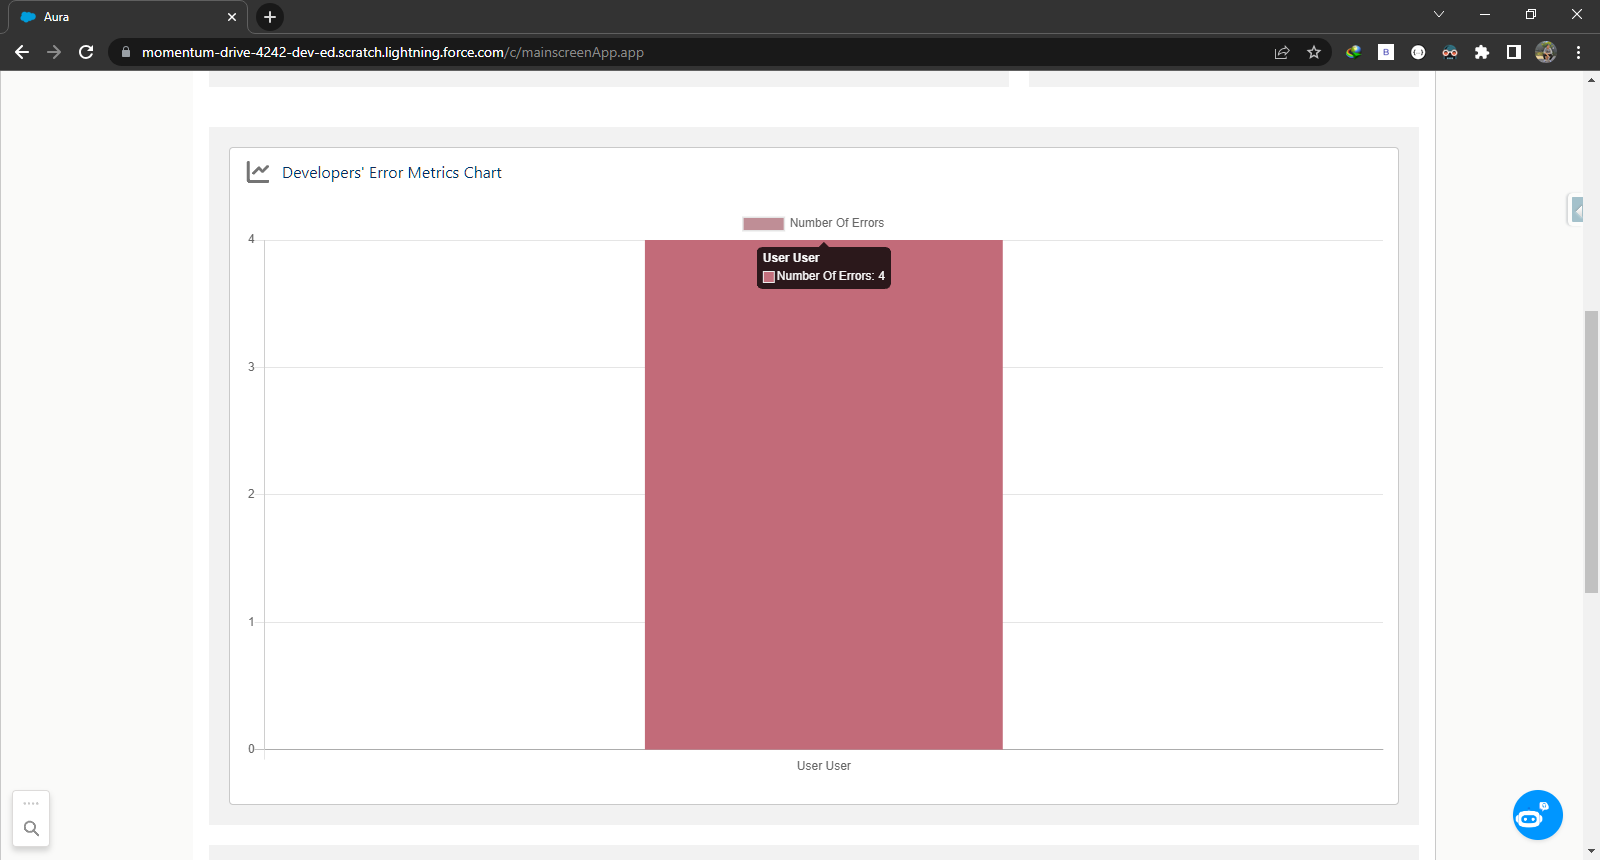
\includegraphics[scale=0.4]{dashboard3.png}
    \caption{Community dashboard interface (developers' error metrics chart)}
\end{figure}
Upon clicking on one of the bars displayed in the previous chart the complete error logs specific to the selected developer will be displayed as shown in the following figure.
\begin{figure}[H]%
    \center   
    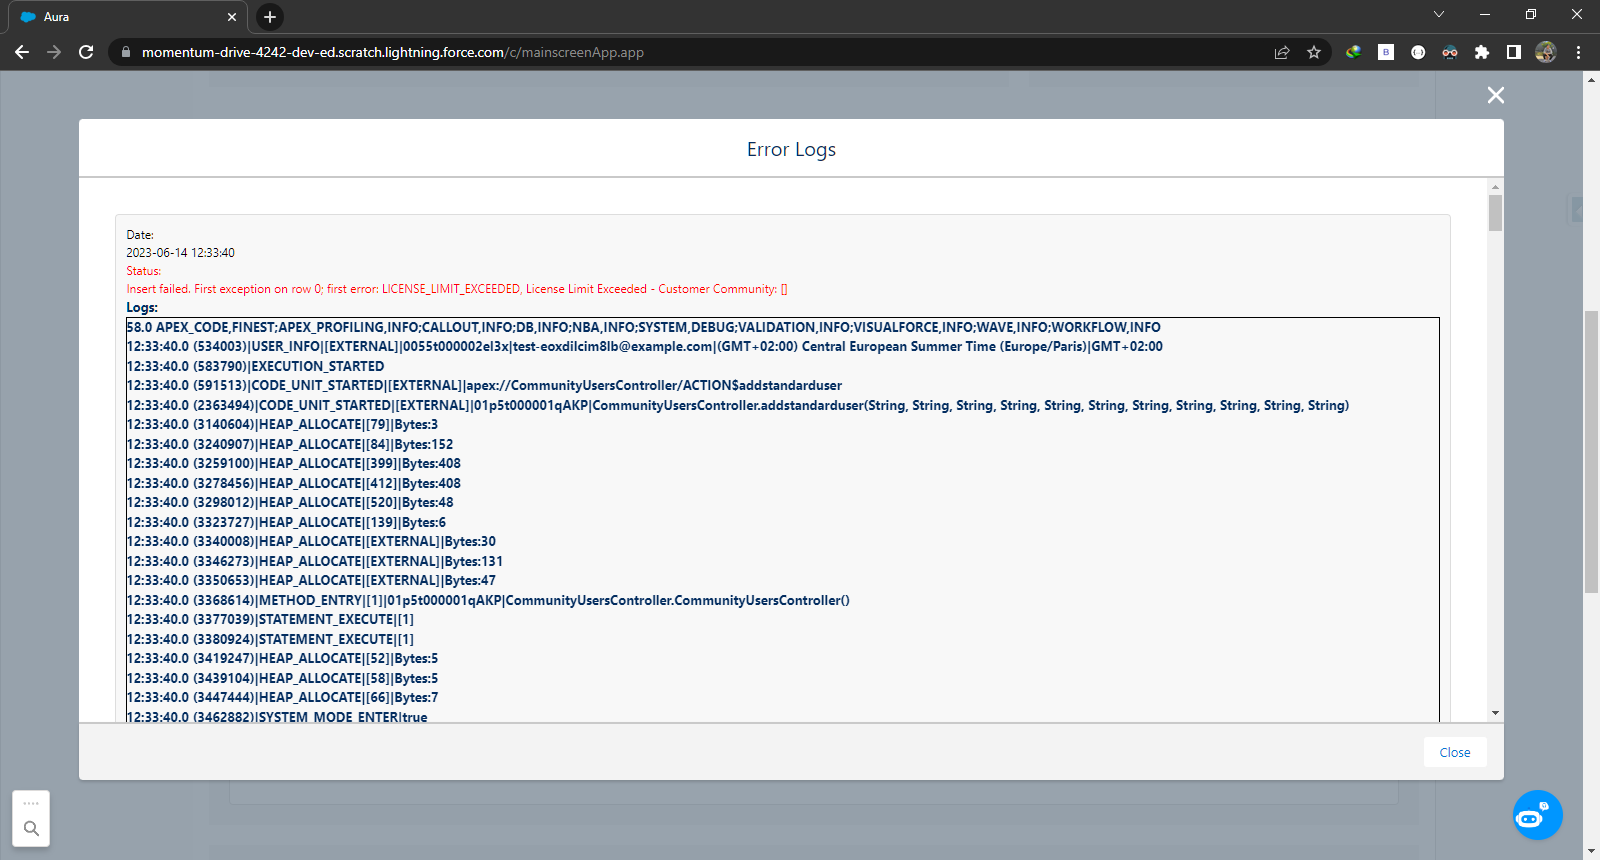
\includegraphics[scale=0.4]{dashboard4.png}
    \caption{Community developer error logs interface}
\end{figure}
\subsection{User list }
The following figure represents the community members list where the user can navigate through his community members' information using given pagination options. He may also filter displayed members by user status (active or inactive), account name, or profile label using the given combo boxes or search for a specific user using his Salesforce user name, full name, or email using the provided search bar. The user can perform actions on one or multiple members, these actions can be activating/deactivating selected members, sending welcome emails to selected members, or sending reset password reset emails to selected members. 

\begin{figure}[H]%
    \center   
    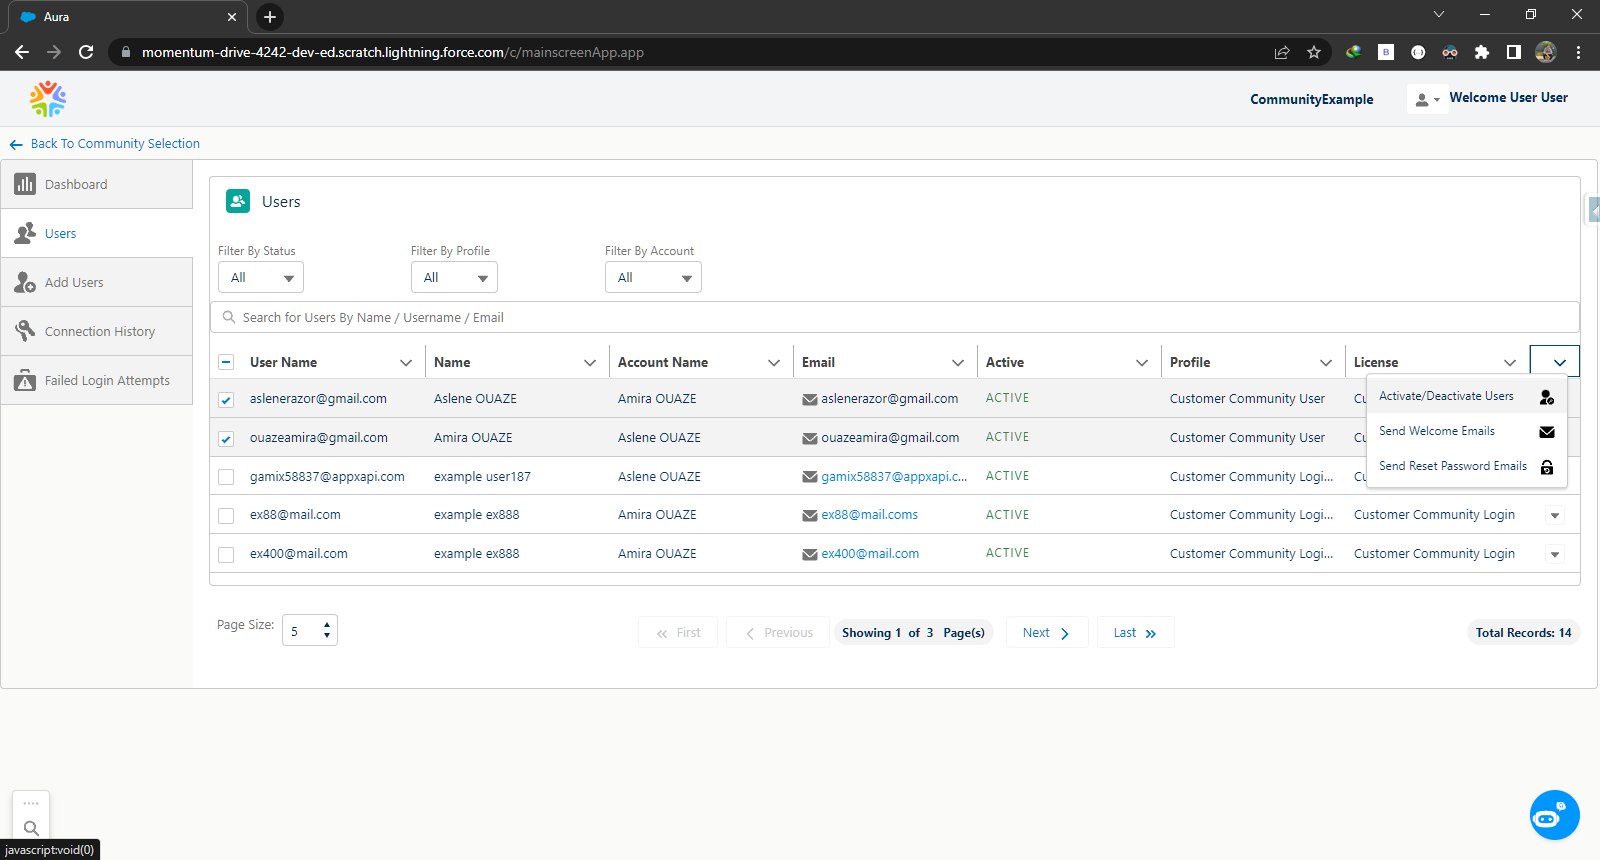
\includegraphics[scale=0.4]{userlist1.png}
    \caption{User list interface}
\end{figure}
The user may also consult details about a specific user as well as update said details as shown in the following figure, the show details action is only selectable when selecting one community member.
\begin{figure}[H]%
    \center   
    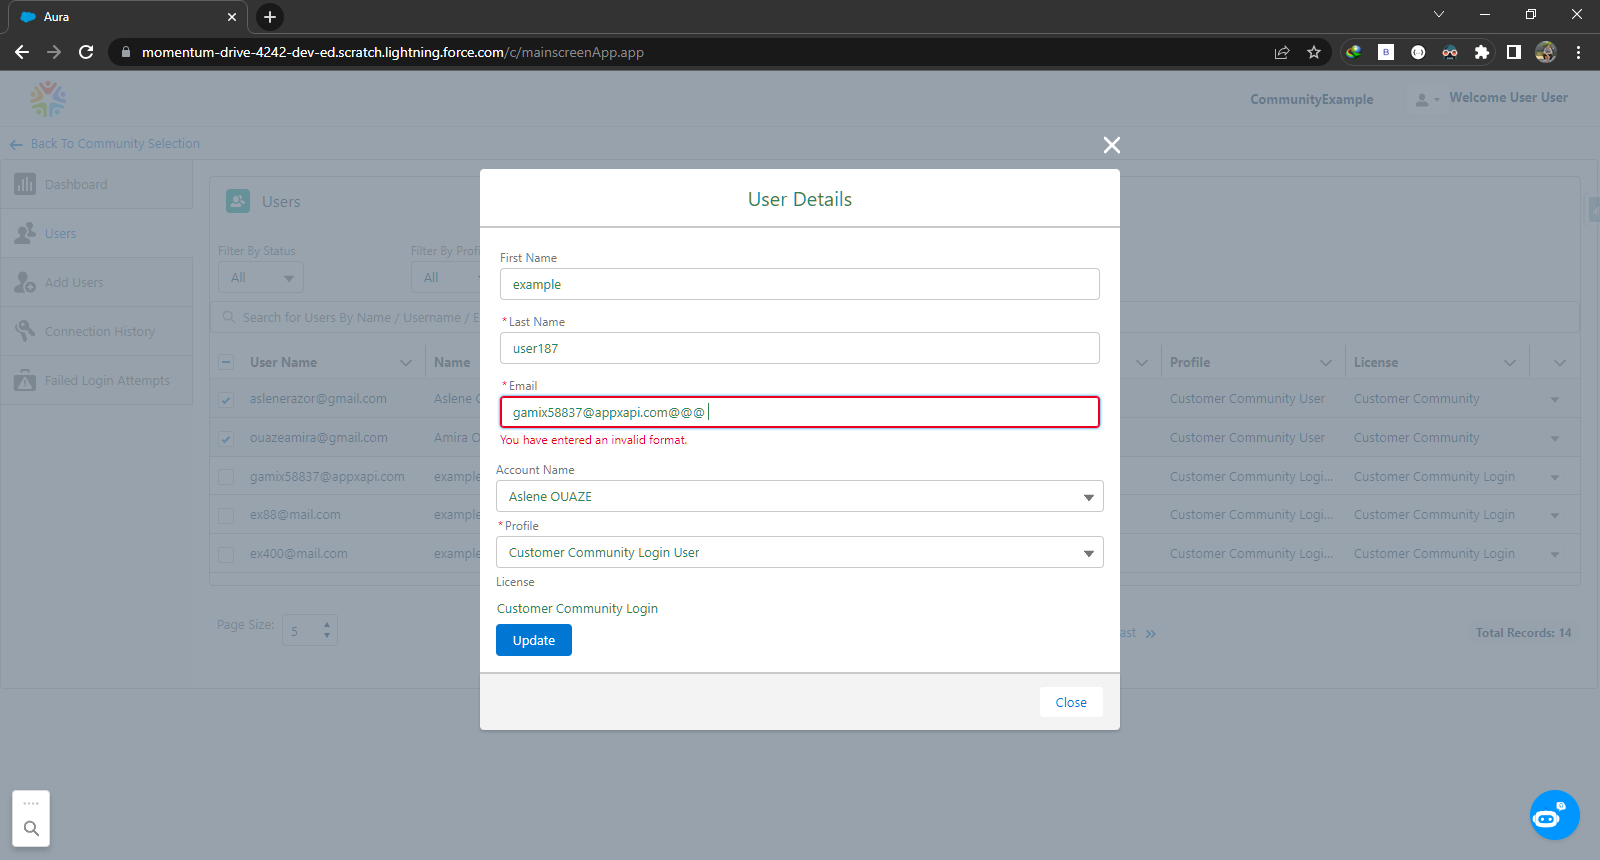
\includegraphics[scale=0.4]{userlist2.png}
    \caption{User details interface}
\end{figure}

\subsection{Add users}
The following figure represents the add users form interface where the user can add one or multiple users using the displayed form fields. The user can fill the initial given form and press the "submit all displayed forms" button where the system will prompt any error message if it exists or the success of the operation otherwise. The user is also able to clone the previously filled form, add a new empty one or delete the latest one using the given buttons.
\begin{figure}[H]%
    \center   
    
    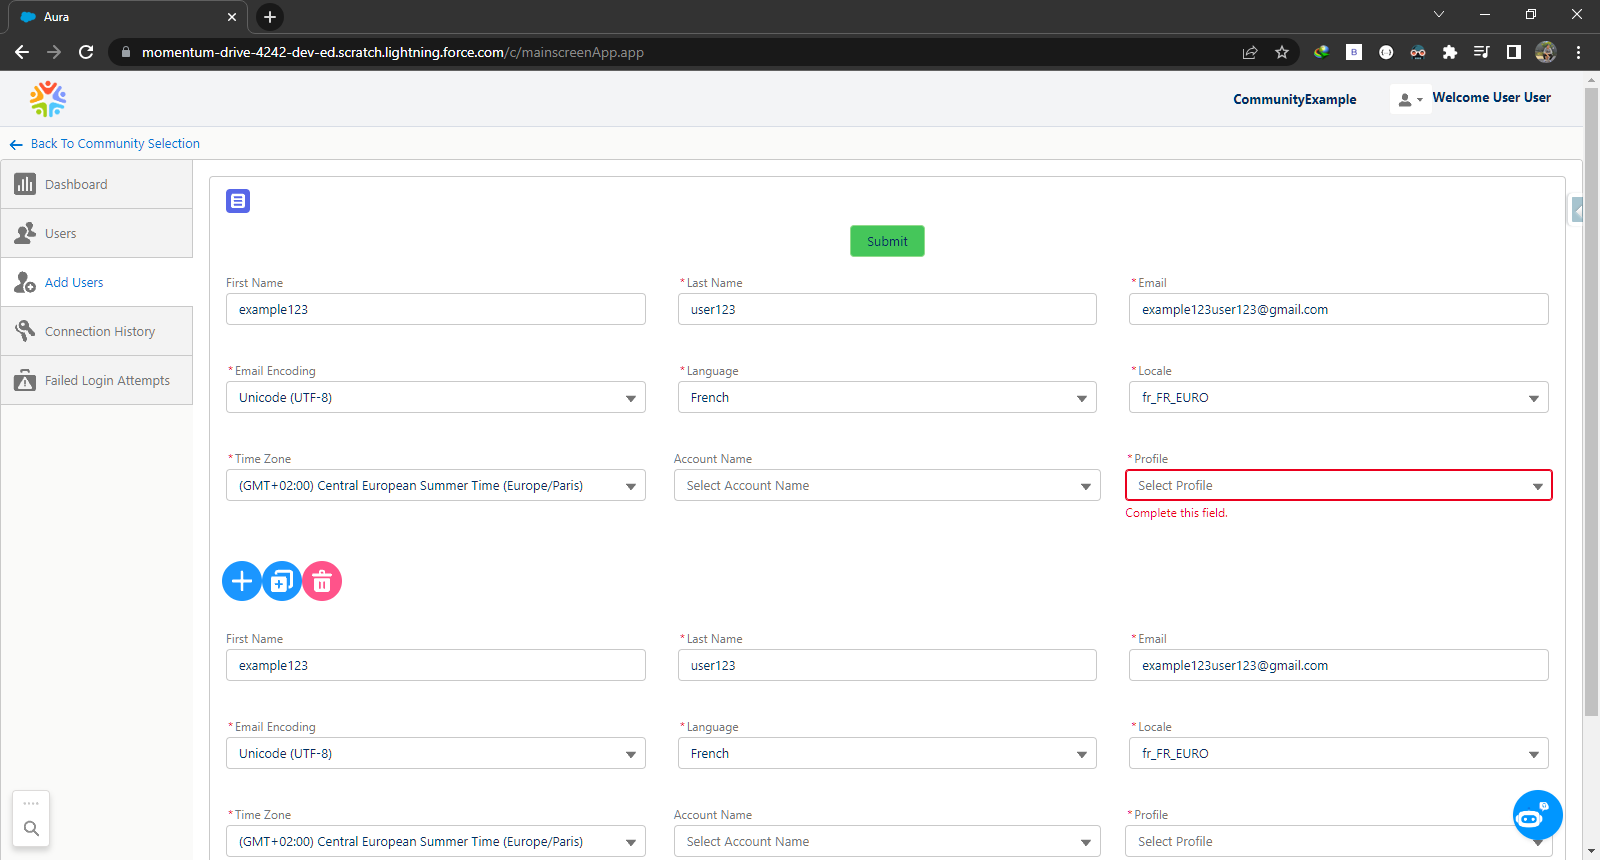
\includegraphics[scale=0.4]{useradd.png}
    \caption{Add users interface}
\end{figure}
\subsection{Connection history}
The following figure represents the connection history interface that shows the number of logins for each user based on the given "from" and "to" dates and time or the time range filter where the user can interact with both of these filters to change the displayed chart.  
\begin{figure}[H]%
    \center   
    
    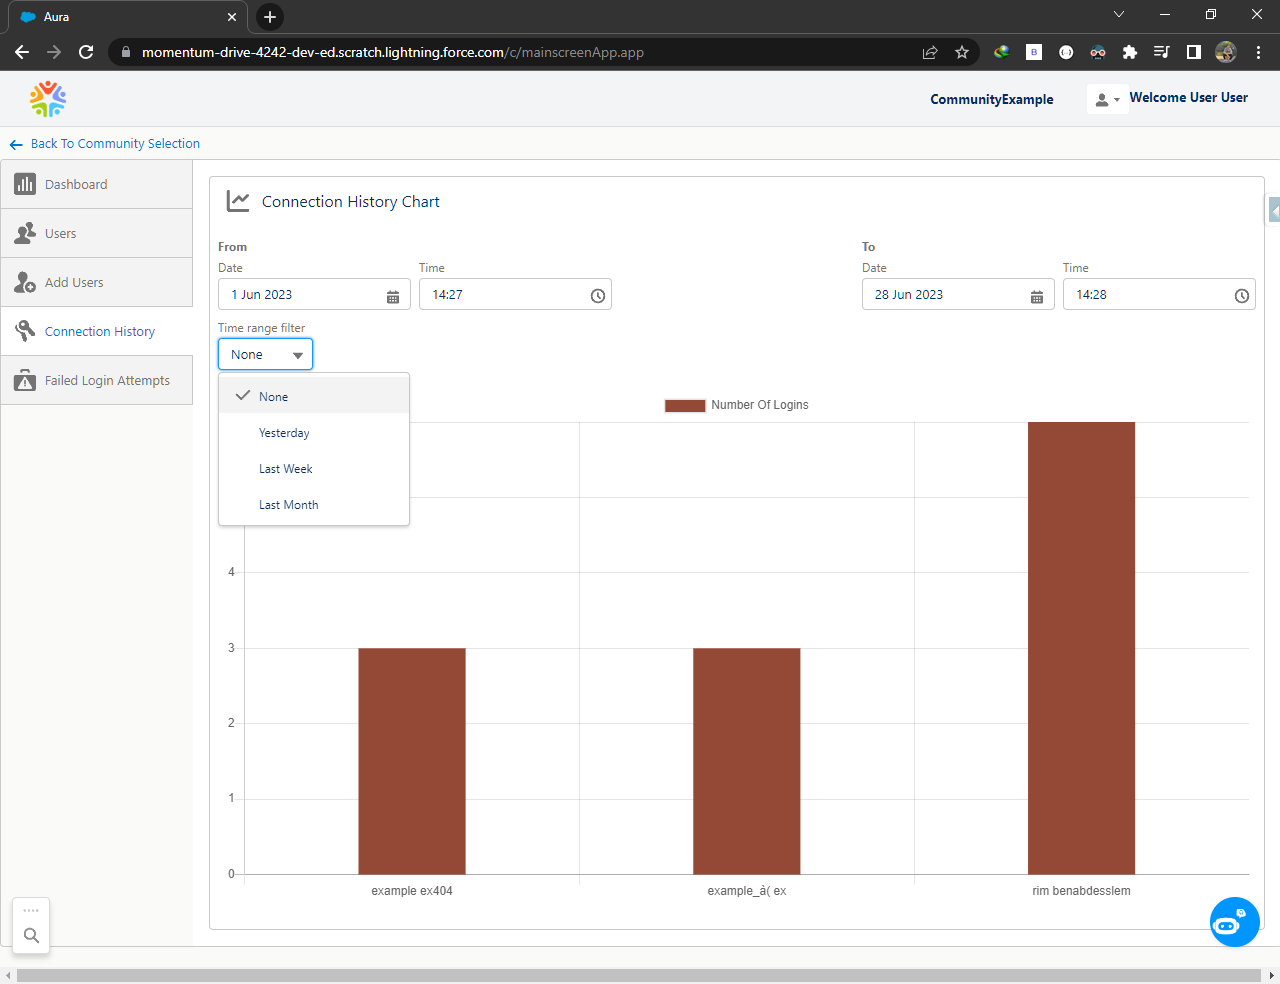
\includegraphics[scale=0.5]{history1.png}
    \caption{Connection history interface (chart)}
\end{figure}
The user may also click one of the displayed bars on the displayed chart to access brief details about the concerned user and update his Salesforce user license as shown in the following figure.
\begin{figure}[H]%
    \center   
    
    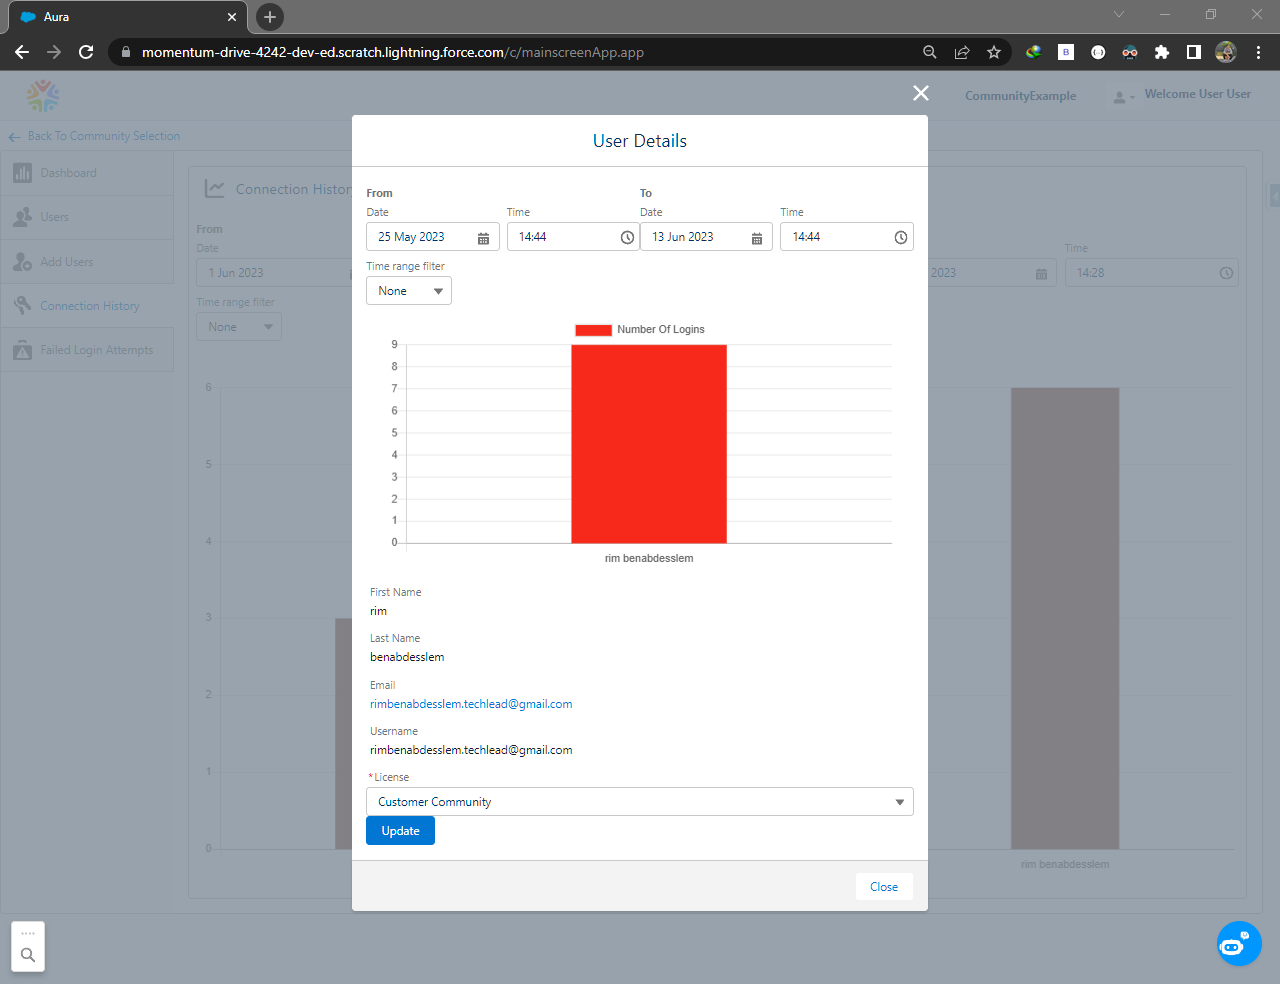
\includegraphics[scale=0.5]{history2.png}
    \caption{Connection history interface (user details)}
\end{figure}
\subsection{Failed login attempts}
The following figure represents the community members' failed login attempts list where the user can navigate through his community login events using given pagination options. He may also filter displayed events by status (invalid password, no community access etc) using the given combo box or search for a specific event using concerned user's Salesforce user name or full name using the provided search bar, he may also filter displayed results by date and time using the provided "from" and "to" filters.\\
The user can also choose to show more details about a specific login event or send a security warning email to the concerned user using the given action menu.

\begin{figure}[H]%
    \center   
    
    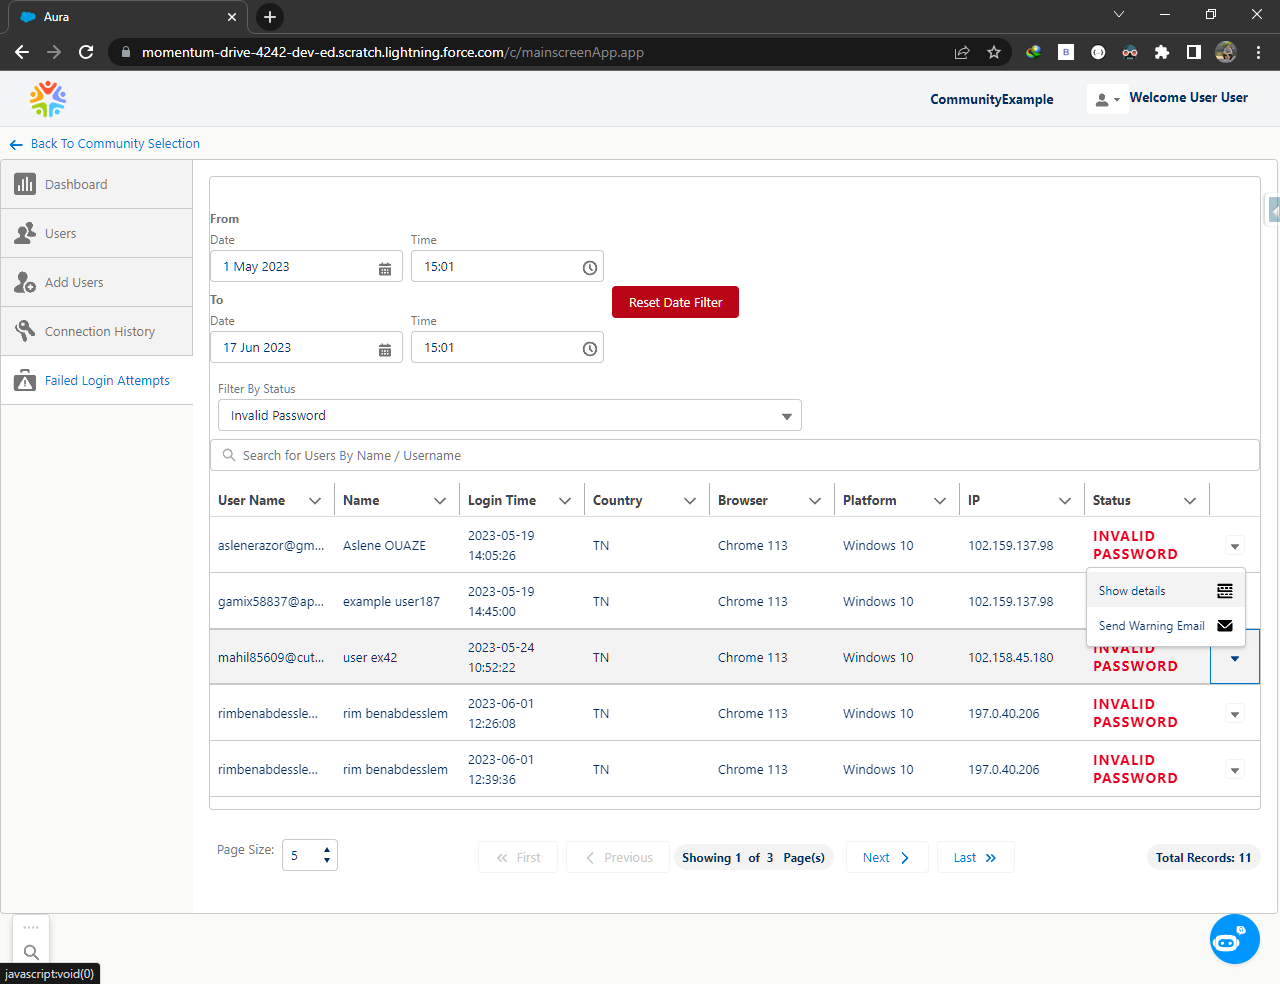
\includegraphics[scale=0.5]{loginattempts1.png}
    \caption{Failed login attempts interface (event list)}
\end{figure}
The following figure represents the selected login event's details interface where the user can navigate the map displaying the event's location in addition to consulting further details about it.
 \begin{figure}[H]%
    \center   
    
    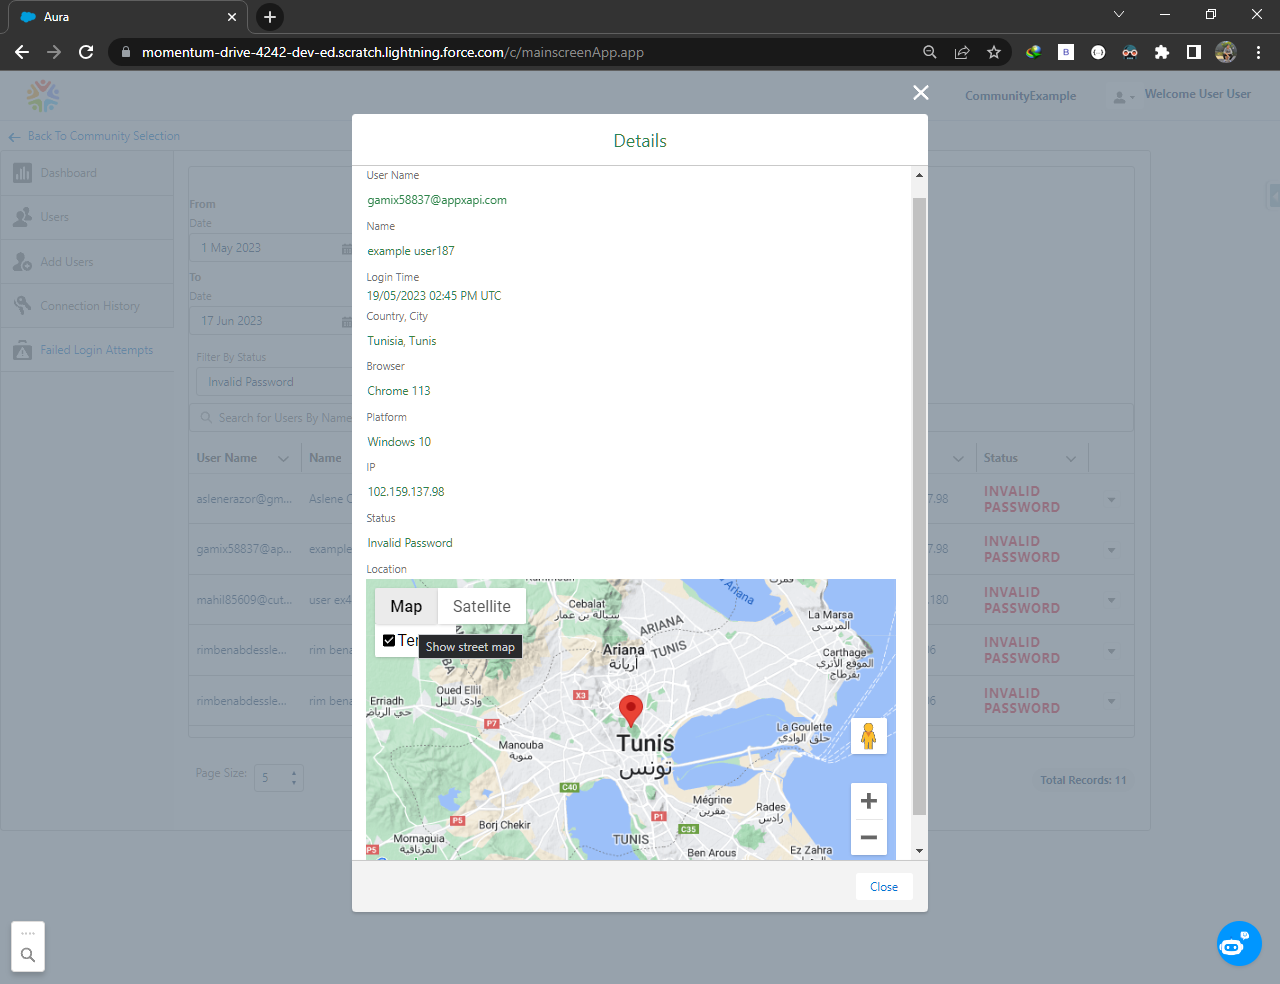
\includegraphics[scale=0.5]{loginattempts2.png}
    \caption{Failed login attempts interface (event details)}
\end{figure}
\subsection{Chatbot}
The following figure represents the Chatbot interface which is accessible from anywhere in the main screen of our application using the floating Chatbot button. In this interface the user may choose one of the predefined questions or type his own question, upon submitting the question the answer will be displayed on screen where the user may choose to give positive or negative feedback to the developers for future improvements.

\begin{figure}[H]%
    \center   
    
    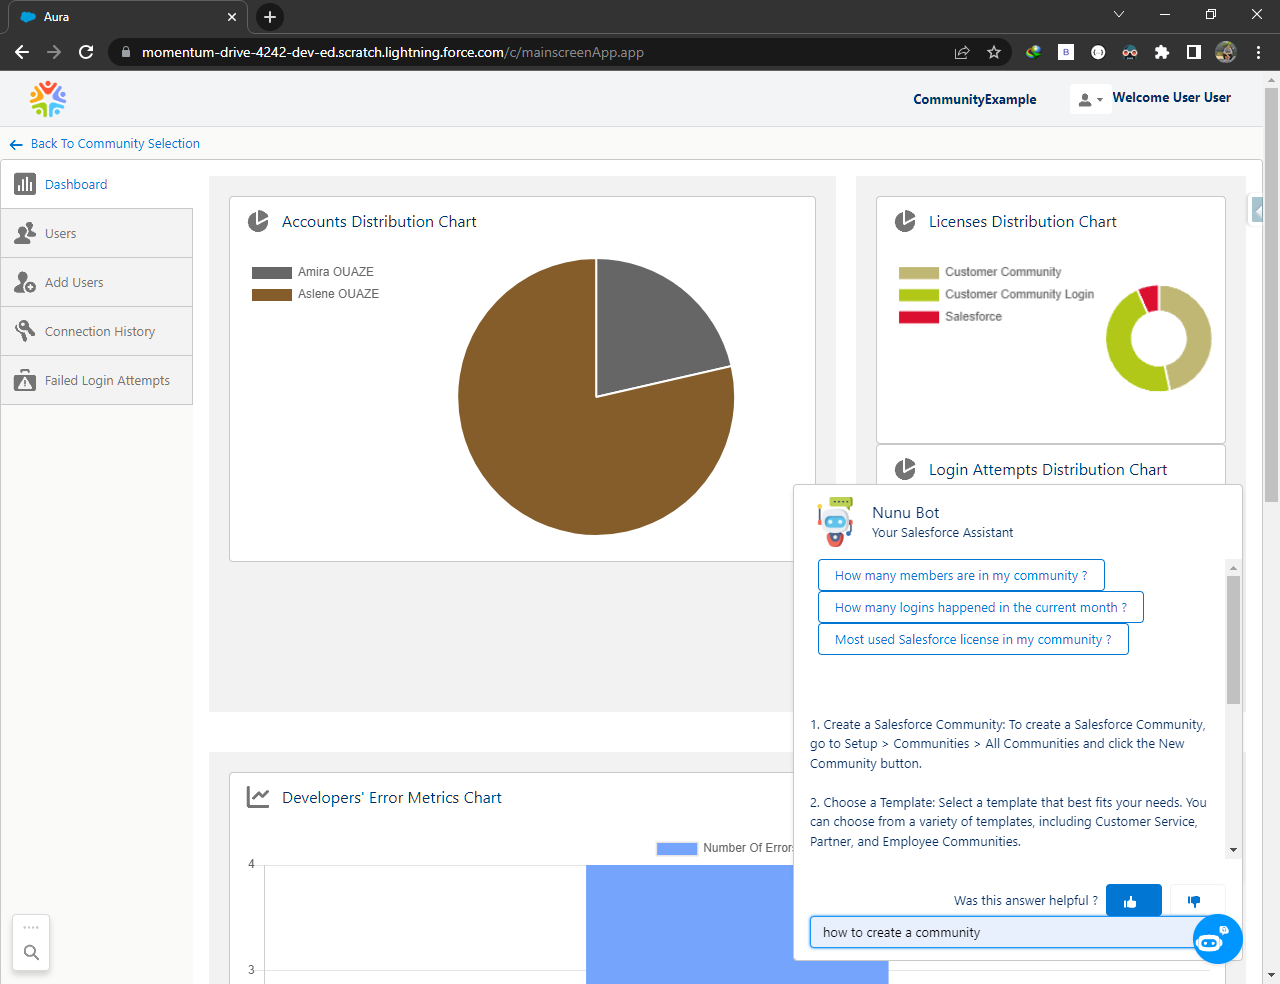
\includegraphics[scale=0.5]{chatbot.png}
    \caption{Chatbot interface}
\end{figure}
\section*{Conclusion}
In this chapter, we presented the technical specification of our
application through the introduction of hardware and software environments. Ultimately,
we have described the features of our application,
illustrated by screenshots of its user interfaces.
We end our report with the general conclusion and the different
prospects.